\documentclass{article}

\usepackage[ngerman]{babel}
\usepackage[utf8]{inputenc}
\usepackage[T1]{fontenc}
\usepackage{hyperref}
\usepackage{csquotes}
\usepackage{graphicx}
\usepackage{float}
\usepackage{caption}

\usepackage[
    backend=biber,
    style=apa,
    sortlocale=de_DE,
    natbib=true,
    url=false,
    doi=false,
    sortcites=true,
    sorting=nyt,
    isbn=false,
    hyperref=true,
    backref=false,
    giveninits=false,
    eprint=false]{biblatex}
\addbibresource{../references/bibliography.bib}

\title{Notizen zum Projekt Data Ethics}
\author{Noah Cooper}
\date{\today}

\begin{document}
\maketitle

\abstract{
    Dieses Dokument ist eine Sammlung von Notizen zu dem Projekt. Die Struktur innerhalb des
    Projektes ist gleich ausgelegt wie in der Hauptarbeit, somit kann hier einfach geschrieben
    werden, und die Teile die man verwenden möchte, kann man direkt in die Hauptdatei ziehen.
}

\tableofcontents

\section{Leifrage}
    Ist es ethisch vertretbar, KI für die Erstellung von Kunst zu verwenden?

\section{Meine Meinung vor der Recherche}
    Mit der KI lassen sich viele interessante Kunstwerke erstellen, wie man anhand von Ai Image 
    Generators erkennen kann. Ich kann mir aber vorstellen, dass viele Künstler*innen eine Gefahr 
    darin sehen, dass ihre Arbeitsplätze und ihre Einnahmequelle verschwinden könnten. Die Kunst der KI 
    hat in meinen Augen ohne den Aspekt der menschlichen Überlegungen nicht so viel Wert. Die KI denkt 
    sich nicht aus, welche Nachricht sie mit ihrer Kunst teilen will, weshalb man sie auch nicht 
    interpretieren und darüber diskutieren kann.

\section{Wie wird KI trainiert?}
    Laut yukosai.com kann das Training einer KI in mehrere Schritte unterteilt werden:
    \begin{enumerate}
        \item Vorbereitung der Trainingsdaten: Auswahl einer großen Anzahl von Bildern als Basis für das Training.
        \item Labeling der Daten: Jedes Bild wird mit entsprechenden Labels versehen, um dem Modell mitzuteilen, welcher Stil oder welches Genre repräsentiert wird.
        \item Aufbau des neuronalen Netzwerks: Das Modell wird so konfiguriert, dass es die gewünschten künstlerischen Merkmale erlernen kann.
        \item Training des Modells: Durch mehrere Iterationen werden die Gewichte im Netzwerk angepasst, um die Genauigkeit und Qualität der generierten Kunstwerke zu verbessern.
        \item Auswertung und Anpassung: Nach dem Training wird das Modell auf seine Leistung überprüft und gegebenenfalls weiter optimiert.
    \end{enumerate}
    ("hier noch mehr schreiben")

\section{Was sagen Befürworter*innen der KI-Kunst?}
    Viele Experten sagen, dass die KI dabei helfen kann, Bedarfe 

\section{Wie gut ist die KI-Kunst?}
    KI Kunst kann sehr verstörend sein, weil sie oft keine richtigen menschlichen Proportionen darstellt.
    \begin{figure}[h]
    \centering
    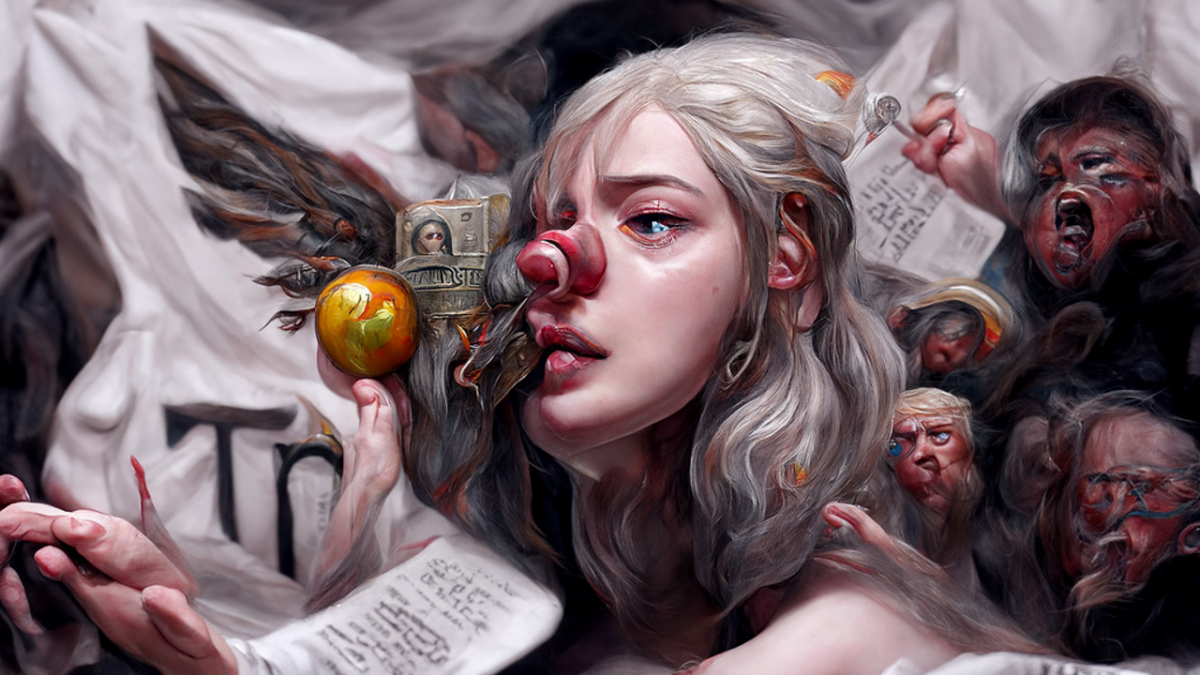
\includegraphics[width=0.8\textwidth]{ki-bild.png} 
    \caption{"A detailed painting of an allegory of truth and lies" - Disco Diffusion (Versuch 55)}
    \label{fig:ki-bild}
    \end{figure}

\input{section_ai.tex}

\printbibliography

\end{document}
